\documentclass[runningheads]{llncs}

\usepackage[T1]{fontenc}
\usepackage[utf8]{inputenc}
\usepackage{hyperref}
\usepackage{url}
\usepackage{amsfonts}
\usepackage{microtype}
\usepackage{txfonts}
\usepackage{xcolor}
\usepackage{amsmath}
\usepackage{caption}
\usepackage{graphicx}
\usepackage{subcaption}
\usepackage{etoolbox}
\usepackage{multicol}
\usepackage[backend=biber, style=nature, sorting=none, doi=false, url=false, eprint=false]{biblatex}
\renewcommand*{\bibfont}{\footnotesize}
\setlength{\columnsep}{5pt}

\addbibresource{prc.bib}

% \title{Conditional diffusion models as  surrogates for physical reservoir computing substrates}
\title{Diffusion models for gradient-based design and optimisation of physical reservoir computing substrates}

\author{Jack Griffiths\inst{1}, Rawana Yagan\inst{2}, Thomas J. Hayward\inst{2} \and Matthew O. A. Ellis\inst{1}}
\authorrunning{J. Griffiths et al.}

\institute{School of Computer Science, University of Sheffield, UK\\
\email{\{jack.griffiths, m.o.ellis\}@sheffield.ac.uk}
\and
School of Chemical, Materials and Biological Engineering, University of Sheffield, UK}

\begin{document}

\maketitle

Physical reservoir computing (RC)~\cite{nakajima2020,markovic2020,allwood2023} exploits the dynamics of a non-linear system as a computational substrate, training only a linear readout. Spintronic systems, such as magnetic domain wall (DW) oscillators~\cite{ababei2021} and interconnected nanomagnetic ring arrays~\cite{vidamour2022}, have been demonstrated as effective RC substrates but singular, monolithic reservoirs can be hard to optimise for a range of desired tasks. Networks of heterogeneous reservoirs can provide richer state representations than individual devices, but optimising such a network requires either costly experimentation or a faithful device model. For fabricated devices a governing equation is rarely available, and capturing the noisy dynamics is essential to minimise the simulation-reality gap~\cite{manneschi2025}. %Here, we learn a surrogate model for such a device from observed trajectories alone, using a conditional denoising diffusion probabilistic model~\cite{ho2020}. 
We use a conditional diffusion model~\cite{ho2020, song2021} to learn surrogates of these devices from experimental output alone; the models are then used for offline training and optimisation of an RC system.

% We seek a generative sampler $g_\phi:(\mathbf{c},\mathbf{z})\mapsto\mathbf{q}$, $\mathbf{z}\sim\mathcal{N}(\mathbf{0},\mathsf{I})$, drawing trajectories $\mathbf{q}\in\mathbb{R}^{N_T}$ from the data distribution $p(\mathbf{q}\mid\mathbf{c})$; the conditioning $\mathbf{c}$ may be a scalar, a parameter vector, or a driving waveform. Clean trajectories $\mathbf{q}_0$ are corrupted toward Gaussian noise over $N_K$ steps; a 1D conditional U-Net $\boldsymbol{\eta}_\phi(\mathbf{q}_k,k,\mathbf{c})$ learns to predict the injected noise by minimising $\mathcal{C}(\phi)=\mathbb{E}_{k,\mathbf{q}_0,\boldsymbol{\eta}} \|\boldsymbol{\eta}-\boldsymbol{\eta}_\phi(\mathbf{q}_k,k,\mathbf{c})\|^2$. Conditioning enters by channel concatenation: scalars are broadcast across time and waveforms are stacked. Inference uses the deterministic DDIM update~\cite{song2021}.

We validate on four systems of increasing complexity, from a pure stochastic process to an experimental substrate: (i) the Ornstein–Uhlenbeck process, which provides a baseline with closed-form moments and autocorrelation; (ii) a driven stochastic Duffing oscillator with combined white and coloured noise, which is non-linear, stochastic, and potentially chaotic, and is conditioned on the driving field amplitude; (iii) a magnetic DW oscillator~\cite{ababei2021} in the collective-coordinate model, which is phenomenologically Duffing-like and forms a physically grounded RC substrate, conditioned on the full driving field; (iv) an experimental interconnected nanomagnetic ring array~\cite{vidamour2022}, conditioned on a rotating in-plane field. Figure~\ref{fig:results} shows trajectories from the diffusion model for each system.
Across all systems, generated ensembles match the held-out data in time-resolved mean, variance, and autocorrelation function. 
%For the OU process the surrogate recovers the analytic moments $\mathbb{E}[q(t)\mid q_0\!=\!0]\!=\!0$ and $\mathrm{Var}[q(t)]\!=\!r(1\!-\!\mathrm{e}^{-2\theta t})$ across $r\!\in\![1/30,3]$. Changing only its conditioning channels, the same U-Net reproduces the Duffing oscillator, DW oscillator, and nanoring statistics.

\begin{figure}[t]
    \centering
    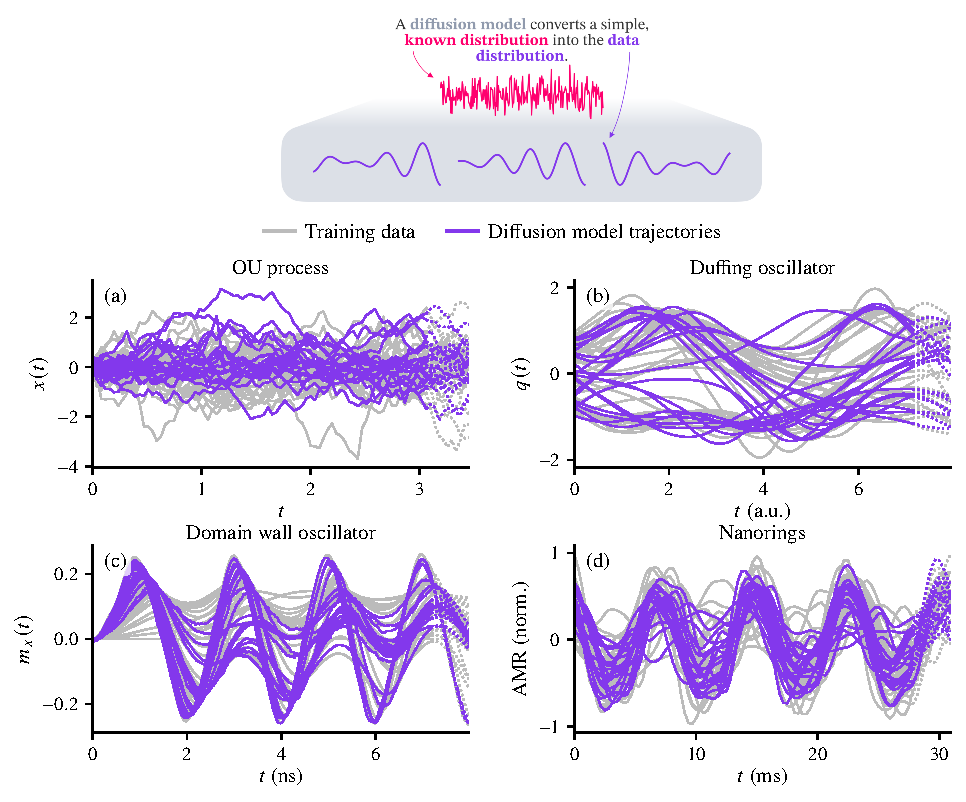
\includegraphics[width=.91\linewidth]{combined_trajectories.pdf}
    \caption{(top) The diffusion model maps a known noise distribution to the trajectory distribution of each substrate. (bottom) Generated trajectories (purple) match the training data (grey) for (a)~the OU process, (b)~the Duffing oscillator, (c)~the DW oscillator, and (d)~experimental nanoring AMR signals.}
    \label{fig:results}
\end{figure}

We demonstrate and exploit the differentiability of 
%$g_\phi$: %
the surrogate models by solving the ill-posed inverse problem of estimating physical parameters by gradient descent from observed trajectories. For example, we can recover the Duffing driving field amplitude with a mean absolute percentage error of $5.74\%\pm3.9\%$, with $95\%$ trials below $12.3\%$ error. Finally, we demonstrate the DW diffusion model as a physical RC substrate for sine-square classification, following the protocol of \cite{ababei2021}. %: the input stream is encoded through a binary mask onto eight virtual nodes, each unique field amplitude spawning a trajectory sampled at equidistant delays.
%A ridge readout %($\lambda=10^{-4}$)%
We achieve $93.6\pm1.4\%$ test classification accuracy (compared to $95\pm5\%$ when using a micromagnetic simulation of the DW~\cite{ababei2021}) which confirms that the surrogate model provides realistic trajectories. %surpassing the $68.75\%$ linear ceiling%The accuracy is robust to the DDIM stochasticity parameter ($93.6\pm1.4\%$ with $\eta=1$, 100~runs),%

These results establish conditional diffusion models as faithful surrogates for spintronic RC substrates, %---and, more generally, for any dynamical system---%
requiring only observed trajectories and no equation of motion, with differentiability opening a route to parameter inference, material design, and optimisation of networks of devices for higher performance physical reservoir computing.

\vspace{-1ex}
{\footnotesize
\printbibliography}

\end{document}